\documentclass[utf8, diplomski, numeric]{fer}
\usepackage{booktabs}
\usepackage[final]{pdfpages}

\begin{document}

% TODO: Navedite broj rada.
\thesisnumber{2981}

% TODO: Navedite naslov rada.
\title{Usporedba algoritama grupiranja u postupcima otkrivanja anomalija}

% TODO: Navedite vaše ime i prezime.
\author{Jelena Nemčić}

\maketitle

% Ispis stranice s napomenom o umetanju izvornika rada. Uklonite naredbu \izvornik ako želite izbaciti tu stranicu.

\includepdf[pages=-]{izvornik.pdf}

% Dodavanje zahvale ili prazne stranice. Ako ne želite dodati zahvalu, naredbu ostavite radi prazne stranice.
\zahvala{}

\tableofcontents

\chapter{Uvod}

Svaki dan generira se velika količina podataka koja se zatim obrađuje kako bi se iz nje saznale nove informacije. Jedan od načina korištenja podataka jest otkrivanje neobičnog ponašanja i pronalaženje anomalija.

Anomalijom se smatra svaki događaj ili opažanje koje značajno odstupa od većine podataka i ne ponaša se na očekivan način. Takvi primjeri mogu izazvati sumnju da ih generira drugačiji mehanizam ili se činiti nedosljednima s ostatkom tog skupa podataka.

Otkrivanje anomalija pronalazi primjenu u mnogim domenama uključujući kibernetičku sigurnost, medicinu, računalni vid, statistiku, neuroznanost i oružane snage. Koristi se također i za otkrivanje financijskih prijevara, industrijskih oštećenja i poremećaja u ekosustavu. Anomalije mogu predstavljati problem te su tada tražene radi namjernog izostavljanja iz skupa podataka kako bi se dobila točnija statistička analiza ili bolje predviđanje nekog modela strojnog učenja. Međutim, u mnogim su primjenama anomalije najzanimiljiviji dio skupa podataka i predstavljaju novu pojavu koju je potrebno identificirati i dalje istražiti.

Jedna od tehnika otkrivanja anomalija jest korištenje algoritama grupiranja s ciljem pronalaženja elemenata koji ne pripadaju niti jednoj grupi. U ovom radu dano je objašnjenje problema pronalaska anomalija, opis različitih algoritama grupiranja i korištenih skupova podataka te usporedba izvedbe tih algoritama u postupcima otkrivanja anomalija. Algoritmi odabrani za usporedbu su K-Means, DBSCAN i Gaussova mješavina, a testirani su na problemima otkrivanja ...


\chapter{Anomalije}
\section{Pojava anomalija i njeni uzroci}
Postoji više pokušaja definiranja anomalija, a većina njih opisuje anomaliju kao opažanje čiji se obrazac ponašanja razlikuje od očekivanog, najčešće se pojavljuje vrlo rijetko u skupu podataka i njegova su obilježja značajno drugačije od onih većine preostalih opažanja. Također, anomalijom se može smatrati podatak koji se čini nedosljedan i relativno udaljen od drugih podataka iz skupa ili izaziva sumnju da ga generira drugačiji mehanizam.

Anomalije se mogu pojaviti u bilo kojem skupu podataka i ponekad njihovo otkrivanje može biti od izuzetne važnosti. Često se otkrivanje anomalija provodi u predobradi kako bi se mogle ukloniti iz skupa podataka. Time se dobiva točnija statistika podataka, bolje predviđanje modela strojnog učenja i bolja vizualizacija podataka. S druge strane, anomalije mogu biti najvažnija i najzanimljivija opažanja i tada se otkrivanje anomalija provodi radi njih samih. Primjeri takve primjene su otkrivanje upada u području kibernetičke sigurnosti, otkrivanje financijskih prijevara i lažnih informacija, otkrivanje kvarova i pogrešaka, praćenje stanja sustava i vremenskih serija, detekciju događaja u senzorskim mrežama, otkrivanje poremećaja u ekosustavu, otkrivanje nedostataka na slikama pomoću računalnog vida te za postavljanje medicinske dijagnoze i provođenje zakona.

Mogući uzroci pojave anomalija su:
\begin{enumerate}
\item Podaci pripadaju različitim razredima.
\begin{itemize}
\item Anomalije se razlikuju od ostalih podataka jer pripadaju drugom razredu, koji ima drugačija obilježja.
\item Primjer takvih anomalija su financijske prijevare, strani upad u sustav i pojava bolesti.
\end{itemize}

\item Prirodna varijacija.
\begin{itemize}
\item Neki skupovi podataka mogu se modelirati normalnom distribucijom, gdje su anomalije oni događaji koji imaju vrlo malu vjerojatnost pojavljivanja.
\end{itemize}

\item Pogreške u mjerenju ili prikupljanju podataka.
\begin{itemize}
\item Do pojave anomalija može doći ako podaci sadrže šum, ako postoji kvar u mjernim instrumentima ili zbog ljudske pogreške.
\item Krajnji je cilj eliminirati ovakve anomalije jer smanjuju kvalitetu podataka.
\end{itemize}

\end{enumerate}

U ovom radu razmatrat će se samo anomalije koje se javljaju kao posljedica toga što podaci prirodno pripadaju različitim razredima.


\section{Klasifikacija anomalija}
Kako bi sustav za otkrivanje anomalija mogao točno identificirati potencijalna odstupanja, nužno je znati koja vrsta anomalije se očekuje. Anomalije se mogu podijeliti u tri glavne kategorije:

\begin{enumerate}
\item Globalne anomalije

Opažanje se smatra globalnim odstupanjem ili globalnom anomalijom ako se njegova vrijednost ili vrijednost nekih njegovih obilježja značajno razlikuje od vrijednosti cjelokupnog skupa podataka. Gledano u n-dimenzionalnom prostoru, taj se podatak nalazi daleko od svih ostalih podataka iz skupa. Primjer globalne anomalije dan je na slici \ref{fig:outlier1}.

\begin{figure}[htb]
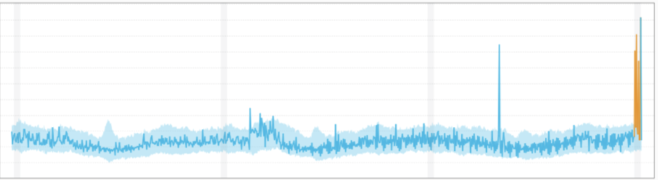
\includegraphics[width=1\textwidth]{images/outlier_type1.png}
\centering
\caption{Globalna anomalija. Preuzeto s  https://towardsdatascience.com/outliers-analysis-a-quick-guide-to-the-different-types-of-outliers-e41de37e6bf6}
\label{fig:outlier1}
\end{figure}

\item Kontekstualne anomalije

Kontekstualne ili uvjetne anomalije su opažanja čije se vrijednosti znatno razlikuju od ostalih opažanja koja postoje u istom kontekstu. Takve vrijednosti ne moraju biti izvan globalnih očekivanja, ali odudaraju od konteksta u kojem se nalaze. Također, jedan podatak koji je anomalija u kontekstu jednog skupa podataka ne mora biti anomalija u drugom. Ovakva odstupanja najčešća su u podacima vremenskih serija jer takvi skupovi podataka sadrže zapise ovisne o vremenskom razdoblju. Slika \ref{fig:outlier2} prikazuje primjer takve anomalije.

\begin{figure}[htb]
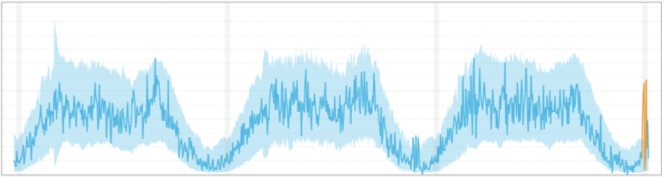
\includegraphics[width=1\textwidth]{images/outlier_type2.png}
\centering
\caption{Kontekstualna anomalija}
\label{fig:outlier2}
\end{figure}

\item Kolektivne anomalije

Podskup podataka smatra se kolektivnom anomalijom ako njihove vrijednosti kao grupa značajno odstupanju od cijelog skupa podataka, ali vrijednosti pojedinačnih podataka nisu same po sebi anomalne ni u globalnom niti u kontekstualnom smislu. U podacima vremenskih serija, kolektivne anomalije mogu se manifestirati kao vrhovi i doline koje se javljaju izvan vremenskog okvira kada je takvo ponašanje normalno, kao što se vidi na slici \ref{fig:outlier3}.

\begin{figure}[htb]
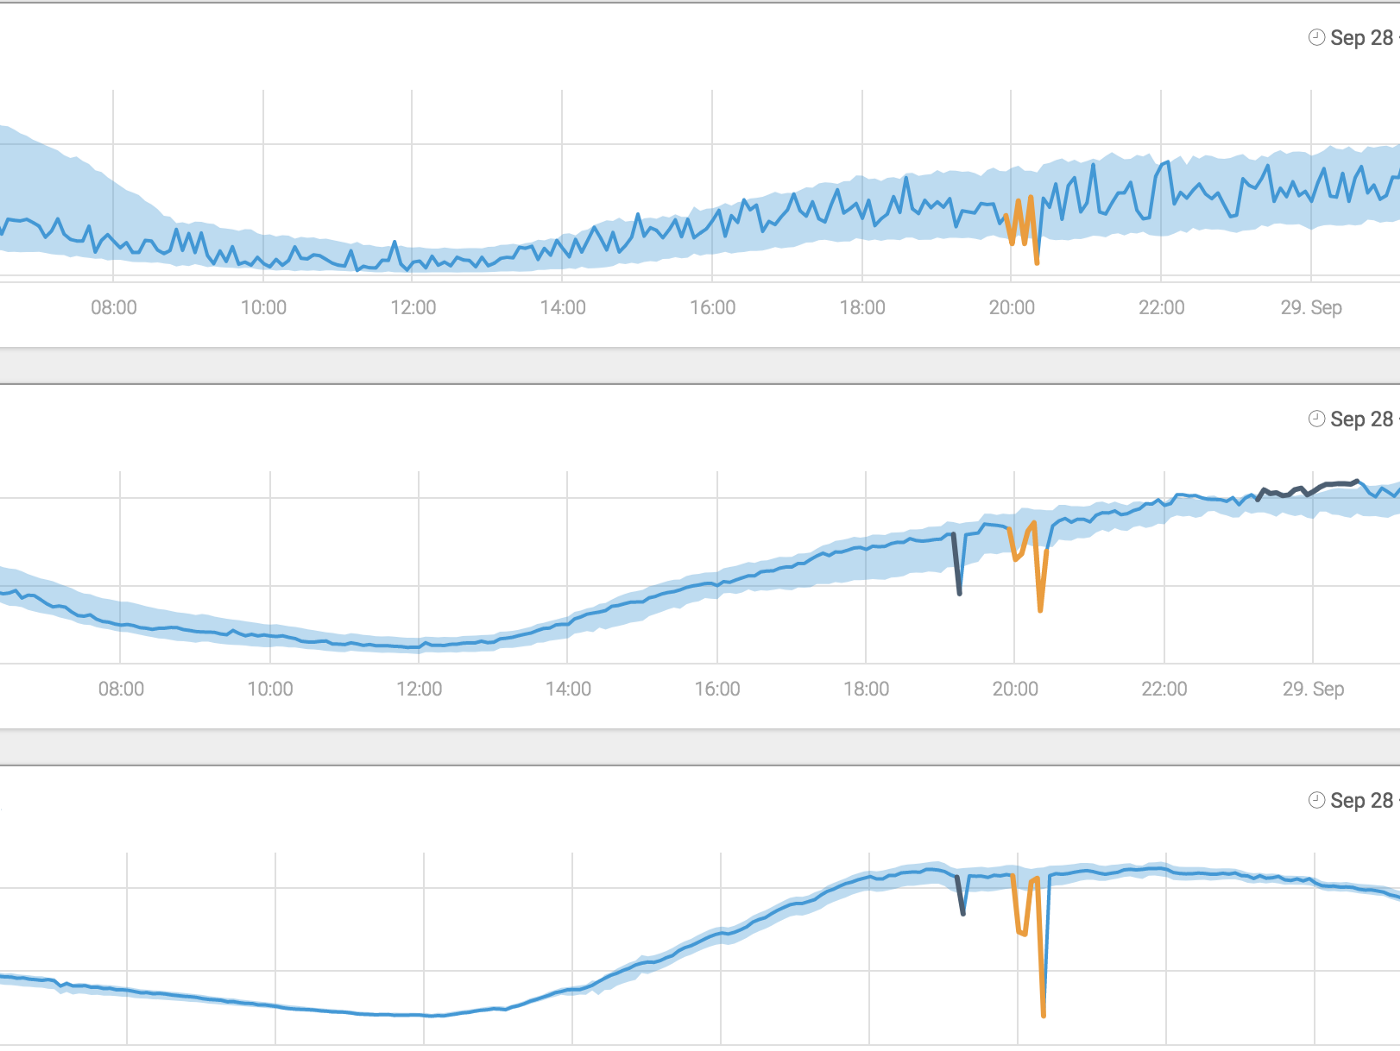
\includegraphics[width=1\textwidth]{images/outlier_type3.png}
\centering
\caption{Kolektivna anomalija}
\label{fig:outlier3}
\end{figure}

\end{enumerate}

Ovisno o vrsti anomalije primjenjuju se različite metode i načini detekcije. Ovaj rad fokusira se na globalne anomalije i njihovo pronalaženje.


\section{Problem otkrivanja anomalija}
Otkivanje anomalija svodi se na problem definiranja očekivanog ponašanja podataka ili granica unutar kojih se podaci smatraju normalnima te identificiranja točaka koje se ne nalaze unutar njih. Postoji nekoliko faktora koji čine ovaj problem vrlo teškim.

\begin{itemize}
\item Učinkovito modeliranje normalnih vrijednosti i ponašanja može biti vrlo izazovan problem. Često je teško nabrojati sva moguća normalna ponašanja nekog objekta i klasificirati neki podatak kao anomaliju. Također, granica  između normalnih podataka i anomalija može biti vrlo nejasna.
\item Svaki problem zahtjeva specifičan način detekcije anomalija jer su odabir mjere sličnosti i modeliranje odnosa ovisni o svojstvima tog problema. Zbog toga nije moguć razvoj univerzalno primjenjive metode otkivanja anomalija.
\item Prikupljeni podaci često sadrže šum koji može imati vrijednosti koje znatno odstupaju od normalnih ili čak nedostaju. Šum smanjuje kvalitetu podataka i otežava definiranje granica između normalnih podataka i anomalija te se često šum može pogrešno identificirati kao anomalija i obrnuto.
\item U nekim primjenama, korisnik ne želi samo identificirati anomalije već i razumjeti zašto su ti podaci detektirani kao abnormalni. Zbog toga metoda otkrivanja anomalija mora biti razumljiva, smislena i pružiti opravdanje detekciji.
\end{itemize}


\section{Metode otkrivanja anomalija}
Postoji puno različitih tehnika otkrivanja anomalija i one se mogu podijeliti u četiri glavne kategorije.

\begin{enumerate}
\item Statističke metode

Statistički pristup naziva se još i pristup temeljen na modelu jer sadrži model koji opisuje obilježja skupa podataka. Model najčešće sadrži distribuciju vjerojatnosti podataka i za svaki podatak računa se vjerojatnost njegova pojavljivanja u tom modelu. Ako je ta vjerojatnost vrlo mala, podatak se proglašava anomalijom.
\item Metode temeljene na blizini
\begin{enumerate}
\item Metode temeljene na udaljenosti

Metode temeljene na udaljenosti pretpostavljaju da je podatak anomalija ako mu se najbliži susjedi nalaze daleko u prostoru značajki odnosno ako blizina objekta njegovim susjedima značajno odstupa od blizine većine drugih objekata njihovim susjedima u istom skupu podataka.
\item Metode temeljene na gustoći

Metode temeljene na gustoći koriste broj podataka koji se nalaze unutar definiranog prostora ispitivanog podatka za definiranje lokalne gustoće. Što je lokalna gustoća objekta manja, veća je vjerojatnost da je on anomalija.
\end{enumerate}
\item Metode temeljene na grupiranju

Metode koje se temelje na grupiranju pretpostavljaju da normalni podaci pripadaju velikim i gustim grupama, dok anomalije pripadaju malim i rijetkim grupama ili ne pripadaju niti jednoj. Razlika između grupiranja i metoda temeljenih na gustoći je u tome što grupiranje dijeli podatke u grupe dok metode temeljene na gustoći dijele podatkovni prostor.
\end{enumerate}
U ovom radu za detekciju anomalija koristit će se algoritmi temeljeni na grupiranju. Za usporedbu su izabrani algoritmi K-Means, DBSCAN i Gaussova mješavina.


\chapter{Algoritmi grupiranja za otkrivanje anomalija}
\section{O algoritmima grupiranja}
Grupiranje je podjela skupa podataka u grupe, tako da su podaci u istoj grupi sličniji jedni drugima nego podacima iz ostalih grupa. Cilj jest pronalaženje intrinzičnih grupa u skupu podataka. Algoritmi grupiranja pripadaju u skupinu nenadziranih metoda strojnog učenja jer su ulazni podaci dani bez ciljnih vrijednosti odnosno nisu označeni. 

Grupiranje se može podijeliti u dvije kategorije:

\begin{enumerate}
\item Tvrdo grupiranje - podatak ili pripada grupi ili ne pripada
\item Meko grupiranje - podatak pripada svakoj grupi s određenom vjerojatnošću
\end{enumerate}

Osim po tipu grupiranja koje provode, algoritmi grupiranja razlikuju se i po tome kako definiraju pojam grupe i sličnost podataka. Svaki algoritam pretpostavlja specifičan model grupe, a najčešći modeli su:

\begin{enumerate}
\item Modeli povezanosti - na temelju udaljenosti podataka stvara se hijerarhijsko stablo grupa 
\item Centroidni modeli - podaci se organiziraju u nehijerarhijske grupe ovisno o udaljenosti od centroida te grupe
\item Modeli distribucije - grupe se modeliraju pomoću vjerojatnosti da podaci pripadaju istoj statističkoj distribuciji
\item Modeli gustoće - područja iste gustoće povezuju se u grupe
\end{enumerate}

Ne postoji objektivno najbolji algoritam grupiranja, već odabir algoritma ovisi o problemu koji se rješava. Algoritam se može odabrati na temelju modela grupe ili eksperimentalno. Također, algoritam dizajniran za jednu vrstu modela grupe općenito neće raditi na skupu podataka koji sadrži drugačiji tip grupa.

Vrednovanje algoritma grupiranja


\section{K-Means}
\section{DBSCAN}
\section{Gaussova mješavina}

\chapter{Korišteni skupovi podataka}
\section{prvi}
\section{drugi}
\section{treći}

\chapter{Implementacija}

\chapter{Rezultati}







\chapter{Zaključak}
Zaključak.

\nocite{*}
\bibliography{literatura}
\bibliographystyle{fer}

\begin{sazetak}
Sažetak na hrvatskom jeziku.

\kljucnerijeci{Ključne riječi, odvojene zarezima.}
\end{sazetak}

% TODO: Navedite naslov na engleskom jeziku.
\engtitle{Title}
\begin{abstract}
Abstract.

\keywords{Keywords.}
\end{abstract}

\end{document}
